% =============================================================================
% ARQUIVO PRINCIPAL — no Overleaf: Main document = main.tex (NAO compile preamble.tex)
% =============================================================================

\PassOptionsToPackage{dvipsnames,svgnames}{xcolor}
\documentclass[12pt]{article}

% =============================================================================
% PREAMBULO — incluido por main.tex via % =============================================================================
% PREAMBULO — incluido por main.tex via % =============================================================================
% PREAMBULO — incluido por main.tex via \input{preamble}
% NAO compile este arquivo sozinho no Overleaf.
% =============================================================================

\usepackage[utf8]{inputenc}
\usepackage{sbc-template}
\usepackage{natbib}
\bibliographystyle{apalike}
%\bibliographystyle{ieeetr}

\usepackage{setspace}
\setstretch{1.15}

\usepackage{geometry}
\geometry{a4paper, portrait, margin=2cm}

% for including figures
\usepackage{graphicx}
\usepackage{caption}
\usepackage{float}
\usepackage{subcaption} % Required for sub-figures

% for drawing
\usepackage{tikz}         % for primitive drawing
\usepackage{pgfplots}     % for data plots
\pgfplotsset{compat=1.18} % suggested by overleaf

% for colors
\usepackage{xcolor}

% for symbols and math
\usepackage{amsmath}
\usepackage{amssymb}
\usepackage{mathtools}
\usepackage{nicefrac,xfrac}

\DeclareMathSymbol{\shortminus}{\mathbin}{AMSa}{"39}

% for some special formatting
\usepackage{ulem}
\usepackage{soul}
\def\ie{i.\@e.\@ } % defining macro for "i.e."

% for algorithms
\usepackage{algorithm}
\usepackage{algpseudocode}
\usepackage{algorithmicx}
\algdef{SE}[SUBALG]{Indent}{EndIndent}{}{\algorithmicend\ }
\algtext*{Indent}
\algtext*{EndIndent}
\renewcommand{\algorithmicrequire}{\textbf{Input:}}
\renewcommand{\algorithmicensure}{\textbf{Output:}}

% for table formatting
\usepackage{hhline}
\usepackage{colortbl}
\usepackage{multicol}
\usepackage{multirow}
\definecolor{SuperHeaderGray}{rgb}{0.825,0.825,0.825}
\definecolor{HeaderGray}{rgb}{0.875,0.875,0.875}
\definecolor{LightHeaderGray}{rgb}{0.925,0.925,0.925}
\definecolor{Grey}{rgb}{0.875,0.875,0.875}
\definecolor{LightGrey}{rgb}{0.95,0.95,0.95}

% for hyperlinks within text
\usepackage[pdftex]{hyperref}
\hypersetup{
  colorlinks=true,
  anchorcolor=black,
  citecolor=blue,%black
  filecolor=black,
  urlcolor=black,
  linkcolor=black
}

% redefining \cite to: blue{[Author, Year]}
\let\oldcite\cite
\renewcommand{\cite}[1]{\textcolor{blue}{[\oldcite{#1}]}}

% redefining references section title to pt-br
\renewcommand{\refname}{Referências}

%% uncomment for linenumbers
% \usepackage{lineno}
% \let\oldequation\equation
% \let\oldendequation\endequation
% \renewenvironment{equation}
%   {\linenomathNonumbers\oldequation}
%   {\oldendequation\endlinenomath}
% \let\olddisplaymath\displaymath
% \let\oldenddisplaymath\enddisplaymath
% \renewenvironment{displaymath}
%   {\linenomathNonumbers\olddisplaymath}
%   {\oldenddisplaymath\endlinenomath}
% \linenumbers

% NAO compile este arquivo sozinho no Overleaf.
% =============================================================================

\usepackage[utf8]{inputenc}
\usepackage{sbc-template}
\usepackage{natbib}
\bibliographystyle{apalike}
%\bibliographystyle{ieeetr}

\usepackage{setspace}
\setstretch{1.15}

\usepackage{geometry}
\geometry{a4paper, portrait, margin=2cm}

% for including figures
\usepackage{graphicx}
\usepackage{caption}
\usepackage{float}
\usepackage{subcaption} % Required for sub-figures

% for drawing
\usepackage{tikz}         % for primitive drawing
\usepackage{pgfplots}     % for data plots
\pgfplotsset{compat=1.18} % suggested by overleaf

% for colors
\usepackage{xcolor}

% for symbols and math
\usepackage{amsmath}
\usepackage{amssymb}
\usepackage{mathtools}
\usepackage{nicefrac,xfrac}

\DeclareMathSymbol{\shortminus}{\mathbin}{AMSa}{"39}

% for some special formatting
\usepackage{ulem}
\usepackage{soul}
\def\ie{i.\@e.\@ } % defining macro for "i.e."

% for algorithms
\usepackage{algorithm}
\usepackage{algpseudocode}
\usepackage{algorithmicx}
\algdef{SE}[SUBALG]{Indent}{EndIndent}{}{\algorithmicend\ }
\algtext*{Indent}
\algtext*{EndIndent}
\renewcommand{\algorithmicrequire}{\textbf{Input:}}
\renewcommand{\algorithmicensure}{\textbf{Output:}}

% for table formatting
\usepackage{hhline}
\usepackage{colortbl}
\usepackage{multicol}
\usepackage{multirow}
\definecolor{SuperHeaderGray}{rgb}{0.825,0.825,0.825}
\definecolor{HeaderGray}{rgb}{0.875,0.875,0.875}
\definecolor{LightHeaderGray}{rgb}{0.925,0.925,0.925}
\definecolor{Grey}{rgb}{0.875,0.875,0.875}
\definecolor{LightGrey}{rgb}{0.95,0.95,0.95}

% for hyperlinks within text
\usepackage[pdftex]{hyperref}
\hypersetup{
  colorlinks=true,
  anchorcolor=black,
  citecolor=blue,%black
  filecolor=black,
  urlcolor=black,
  linkcolor=black
}

% redefining \cite to: blue{[Author, Year]}
\let\oldcite\cite
\renewcommand{\cite}[1]{\textcolor{blue}{[\oldcite{#1}]}}

% redefining references section title to pt-br
\renewcommand{\refname}{Referências}

%% uncomment for linenumbers
% \usepackage{lineno}
% \let\oldequation\equation
% \let\oldendequation\endequation
% \renewenvironment{equation}
%   {\linenomathNonumbers\oldequation}
%   {\oldendequation\endlinenomath}
% \let\olddisplaymath\displaymath
% \let\oldenddisplaymath\enddisplaymath
% \renewenvironment{displaymath}
%   {\linenomathNonumbers\olddisplaymath}
%   {\oldenddisplaymath\endlinenomath}
% \linenumbers

% NAO compile este arquivo sozinho no Overleaf.
% =============================================================================

\usepackage[utf8]{inputenc}
\usepackage{sbc-template}
\usepackage{natbib}
\bibliographystyle{apalike}
%\bibliographystyle{ieeetr}

\usepackage{setspace}
\setstretch{1.15}

\usepackage{geometry}
\geometry{a4paper, portrait, margin=2cm}

% for including figures
\usepackage{graphicx}
\usepackage{caption}
\usepackage{float}
\usepackage{subcaption} % Required for sub-figures

% for drawing
\usepackage{tikz}         % for primitive drawing
\usepackage{pgfplots}     % for data plots
\pgfplotsset{compat=1.18} % suggested by overleaf

% for colors
\usepackage{xcolor}

% for symbols and math
\usepackage{amsmath}
\usepackage{amssymb}
\usepackage{mathtools}
\usepackage{nicefrac,xfrac}

\DeclareMathSymbol{\shortminus}{\mathbin}{AMSa}{"39}

% for some special formatting
\usepackage{ulem}
\usepackage{soul}
\def\ie{i.\@e.\@ } % defining macro for "i.e."

% for algorithms
\usepackage{algorithm}
\usepackage{algpseudocode}
\usepackage{algorithmicx}
\algdef{SE}[SUBALG]{Indent}{EndIndent}{}{\algorithmicend\ }
\algtext*{Indent}
\algtext*{EndIndent}
\renewcommand{\algorithmicrequire}{\textbf{Input:}}
\renewcommand{\algorithmicensure}{\textbf{Output:}}

% for table formatting
\usepackage{hhline}
\usepackage{colortbl}
\usepackage{multicol}
\usepackage{multirow}
\definecolor{SuperHeaderGray}{rgb}{0.825,0.825,0.825}
\definecolor{HeaderGray}{rgb}{0.875,0.875,0.875}
\definecolor{LightHeaderGray}{rgb}{0.925,0.925,0.925}
\definecolor{Grey}{rgb}{0.875,0.875,0.875}
\definecolor{LightGrey}{rgb}{0.95,0.95,0.95}

% for hyperlinks within text
\usepackage[pdftex]{hyperref}
\hypersetup{
  colorlinks=true,
  anchorcolor=black,
  citecolor=blue,%black
  filecolor=black,
  urlcolor=black,
  linkcolor=black
}

% redefining \cite to: blue{[Author, Year]}
\let\oldcite\cite
\renewcommand{\cite}[1]{\textcolor{blue}{[\oldcite{#1}]}}

% redefining references section title to pt-br
\renewcommand{\refname}{Referências}

%% uncomment for linenumbers
% \usepackage{lineno}
% \let\oldequation\equation
% \let\oldendequation\endequation
% \renewenvironment{equation}
%   {\linenomathNonumbers\oldequation}
%   {\oldendequation\endlinenomath}
% \let\olddisplaymath\displaymath
% \let\oldenddisplaymath\enddisplaymath
% \renewenvironment{displaymath}
%   {\linenomathNonumbers\olddisplaymath}
%   {\oldenddisplaymath\endlinenomath}
% \linenumbers


\begin{document}

\title{
Trabalho de Álgebra Linear Computacional \hspace{2.0ex} 26.1\\
Compressão de tokens em embeddings via SVD e leverage scores
}

\author{
    Nome Sobrenome\inst{1}
}

\address{
    Instituto de Computação -- Universidade Federal Fluminense (UFF)\\
    Niterói -- RJ -- Brasil -- 24210-346
    \email{pessoa@id.uff.br}
}
\maketitle

\begin{abstract}
Modelos de linguagem de grande porte (LLMs) processam sequências longas de tokens, o que eleva custo de memória e tempo de inferência. Neste artigo, estudamos compressão de embeddings textuais via \textbf{SVD truncada com leverage scores}, inspirada no SVD-Prune: dada $F \in \mathbb{R}^{T \times D}$ (hidden states token-level), selecionamos $T' \ll T$ linhas no subespaço dominante. Desenvolvemos fundamentação (Gram--Schmidt, espectral, $F^\top F$ PSD, leverage clássico e ponderado), implementamos pipeline reprodutível com baseline \texttt{random} e comparamos operadores SVD em reviews IMDb ($\approx$400 amostras, $\bar{T}\approx 209$ tokens) em grade $\varepsilon \times \rho$ ($3 \times 3$). Medimos perda de informação por dois proxies: compressão $C$ e energia espectral $E_k^{\mathrm{energia}}$ (algébrico), e acurácia de sentimento com classificador ridge sobre embeddings podados (supervisionado). A SVD beneficia-se de $\varepsilon$ mais alto e supera o teto em compressão moderada, mas \texttt{svd\_energia} degrada em compressão agressiva.
\end{abstract}

\noindent\textit{\textbf{Palavras-chave}}: SVD, leverage scores, compressão de tokens, embeddings, álgebra linear computacional.

\section{Introdução}\label{sec:intro}

Modelos baseados em Transformers representam a entrada (prompt, documento anexado ou histórico de agente) como uma \textbf{sequência de tokens} processada camada a camada via \emph{self-attention}. Cada token ocupa espaço na janela de contexto e contribui para o custo de inferência, que em atenção densa escala de forma superlinear com o comprimento da sequência\footnote{Em atenção densa, cada token interage com todos os demais; o custo de computação e memória cresce mais rápido que $T$ (tipicamente $O(T^2)$), e não de forma proporcional ($O(T)$).}. Em aplicações com contexto longo (sumarização, RAG, agentes autônomos), boa parte do orçamento de tokens é consumida antes da resposta final: leituras exploratórias, buscas e trechos irrelevantes permanecem no histórico e são reprocessados a cada passo \cite{zhang2026fastcontext,chen2024fastv}.

Evidências recentes quantificam esse gargalo. Zhang \emph{et al.} \cite{zhang2026fastcontext} observam que, em agentes de codificação, leitura e busca consomem cerca de \textbf{46{,}5\%} dos tokens do agente principal; trajetórias end-to-end podem atingir centenas de milhares a milhões de tokens antes de uma correção ser proposta. Separar exploração e devolver contexto compacto reduz o consumo em até \textbf{60\%}, sem degradar (e por vezes melhorando) a taxa de resolução. Benchmarks de \emph{token pruning} em modelos multimodais indicam que muitos tokens carregam pouca informação nova \cite{chen2024fastv,yang2024visionzip}. Comprimir ou selecionar tokens é, portanto, central para custo e qualidade do raciocínio downstream.

Uma linha de trabalho aborda o problema pela \textbf{estrutura algébrica} da matriz de \emph{features} $F \in \mathbb{R}^{T \times D}$ (uma linha por unidade vetorizada, $D$ dimensões por embedding), em vez de heurísticas puramente locais. O SVD-Prune \cite{apedo2026svdprune} critica métodos guiados apenas por scores de atenção: esses pesos tendem a favorecer tokens no início e no fim da sequência (máscara causal, codificação posicional, padrões de leitura), ranqueando tokens menos relevantes quando o orçamento de poda é pequeno. A abordagem decompõe $F$ por SVD, seleciona um subespaço dominante por energia espectral e ranqueia cada token por \emph{leverage scores} das linhas de $U_k$.

Adotamos a SVD \textbf{por documento} (por sequência), e não sobre um corpus agregado: cada texto produz sua matriz $F$; a decomposição identifica modos dominantes \emph{dentro} dessa sequência e os leverage scores ranqueiam tokens \emph{dela}. Isso espelha o uso em inferência: poda de prompt, contexto anexado ou histórico de agente ocorre \textbf{antes} de processar aquela instância, sem acesso a um universo de documentos. Não empilhamos linhas de reviews distintas numa matriz corpus-wide: tal agregação misturaria textos independentes e responderia a outra pergunta (estrutura \textbf{entre} documentos, não poda no eixo sequencial $T \to T'$). A justificativa formal está na Seção~\ref{sec:svd-por-documento}.

Neste relatório de Álgebra Linear Computacional (ALC), isolamos esse operador e comparamos, sob orçamento fixo $\rho$, variantes SVD (\texttt{svd}, \texttt{svd\_energia}) com o baseline \texttt{random}. A pergunta empírica é se seleção por leverage score preserva mais sinal útil do que poda aleatória quando mantemos apenas uma fração $T' \ll T$ das linhas de $F$.

Para quantificar perda de informação, materializamos o fluxo \textbf{texto $\to$ embedding $F$ $\to$ poda $\to$ avaliação} sobre \textbf{reviews longas do IMDb} ($\approx$400 amostras, $\bar{T}\approx 209$ tokens): textos redundantes, sentimento binário supervisionado e comprimento compatível com a motivação de compressão. Cada operador reduz $F$ a $F[S,:]$; treino e teste passam pela mesma poda antes de qualquer medição (Seção~\ref{sec:pipeline}). Usamos dois proxies complementares:
\begin{itemize}
    \item \textbf{Algébrico}: compressão $C$ e, para métodos SVD, energia espectral $E_k^{\mathrm{energia}}$ do subespaço truncado;
    \item \textbf{Supervisionado}: acurácia de sentimento após pooling médio das linhas podadas, normalização $L_2$ e classificador ridge; \texttt{full} (sem poda) serve de teto.
\end{itemize}
Consideramos \emph{menor perda} quando, à compressão equivalente, a acurácia se aproxima mais de \texttt{full} do que nas heurísticas comparadas. Interpretamos o encadeamento teórico (Gram--Schmidt, espectral, $F^\top F$, posto) \cite{alc21svd,alc19espectral,alc11base}; não replicamos agentes nem VLMs completos, e os proxies medem degradação do operador algébrico, não equivalência de saída generativa.

A Seção~\ref{sec:fundamentacao} desenvolve a base teórica; a Seção~\ref{sec:metodologia} detalha o pipeline; a Seção~\ref{sec:resultados} apresenta as comparações empíricas.

\section{Fundamentação teórica}\label{sec:fundamentacao}

\subsection{Sequência, features e problema de poda}\label{sec:contexto-f}

Em modelos baseados em Transformers, o custo de inferência cresce com o comprimento da sequência processada --- em atenção densa, de forma superlinear em $T$ \cite{chen2024fastv}. Técnicas de \emph{pruning} procuram reduzir o número de unidades de contexto antes ou durante a inferência. Formalmente, representamos essas unidades por uma matriz de \emph{features} $F$, cujas linhas são candidatas à poda.

Consideremos uma sequência de $T$ vetores $\mathbf{f}_1, \ldots, \mathbf{f}_T \in \mathbb{R}^D$, empilhados como linhas de
$$
F = \begin{bmatrix} \mathbf{f}_1^\top \\ \mathbf{f}_2^\top \\ \vdots \\ \mathbf{f}_T^\top \end{bmatrix} \in \mathbb{R}^{T \times D}.
$$
Cada linha de $F$ representa uma \textbf{unidade de contexto já vetorizada} --- por exemplo, um \emph{vision token} em VLMs \cite{apedo2026svdprune}, um token textual em camada intermediária de um Transformer, ou um \emph{chunk} (trecho de documento, bloco de código) representado por embedding. A SVD \textbf{não} opera sobre texto bruto nem sobre identificadores discretos do tokenizer; opera sobre representações vetoriais contínuas. Neste relatório, $F$ denota genericamente essa matriz de features; a metodologia (Seção~\ref{sec:metodologia}) especifica embeddings de tokens textuais via \texttt{all-MiniLM-L6-v2} e matrizes sintéticas de posto controlado.

\paragraph{Objetivo da poda.}
Dado orçamento $T' \leq T$, buscamos $S \subset \{1, \ldots, T\}$, $|S| = T'$, e a submatriz $F[S,:] \in \mathbb{R}^{T' \times D}$. A compressão nos experimentos é
$$
C = 1 - \frac{T'}{T}.
$$
O objetivo final é reduzir o eixo de sequência ($T \to T'$), preservando a dimensão $D$ das linhas mantidas. Internamente, a SVD projeta $F$ em um subespaço de dimensão $k \ll \min(T,D)$ para estimar importância estrutural das linhas.

O problema central é escolher $S$ de forma que $F[S,:]$ preserve informação útil para tarefas downstream --- \textbf{sem depender exclusivamente} de heurísticas locais, posicionais ou específicas de uma camada de atenção \cite{apedo2026svdprune}. Abordagens semânticas em agentes (p.ex.\ FastContext \cite{zhang2026fastcontext}) selecionam trechos por relevància à tarefa; aqui estudamos um critério \textbf{algébrico} sobre $F$, complementar à seleção semântica.

\paragraph{Adaptação conceitual.}
Embora a formulação seja inspirada em \emph{token pruning} interno (SVD-Prune em VLMs), a mesma estrutura matricial pode ser reinterpretada em nível de \emph{chunks} ou arquivos, desde que cada unidade seja um vetor. Não reproduzimos um VLM nem um agente de codificação completo; avaliamos o operador em embeddings token-level de reviews IMDb (sequências mais longas que notícias curtas) para aproximar a motivação de compressão de contexto redundante.

\subsection{Posto efetivo e decaimento espectral}

Em sequências redundantes, várias linhas de $F$ são combinações lineares (ou quase) de poucas direções dominantes. Em dados reais, \textbf{não} se espera necessariamente posto algébrico baixo: $\mathrm{rank}(F)$ pode ser $\min(T,D)$, mas a \textbf{energia espectral}
$$
\|F\|_F^2 = \sum_{j=1}^{r} \sigma_j^2
$$
concentra-se nos primeiros valores singulares --- cenário de \textbf{posto efetivo} $r_{\mathrm{eff}} \ll \min(T,D)$ sob critério numérico \cite{alcposto,alc21svd}. Modos com $\sigma_j$ pequenos contribuem pouco à reconstrução; isso motiva aproximação de posto baixo e seleção de linhas no subespaço dominante.

\subsection{Bases ortonormais e decomposição espectral}

O ponto relevante de \textbf{Gram--Schmidt} \cite{alc11base} não é o algoritmo em si, mas substituir um conjunto redundante por uma \textbf{base ortonormal} do mesmo subespaço: dado $\{v_1,\ldots,v_k\}$ linearmente independentes, obtém-se $\{q_1,\ldots,q_k\}$ com $q_i^\top q_j = \delta_{ij}$ e $\mathrm{span}\{q_1,\ldots,q_k\} = \mathrm{span}\{v_1,\ldots,v_k\}$ \cite{alc04produto}.

Para matrizes \textbf{simétricas} $A \in \mathbb{R}^{n \times n}$, o teorema espectral \cite{alc19espectral} garante $A = Q \Lambda Q^\top$, com $Q$ ortogonal e $\Lambda = \mathrm{diag}(\lambda_1,\ldots,\lambda_n)$, $\lambda_1 \geq \cdots \geq \lambda_n$. Se $A$ é \textbf{PSD}, todos os $\lambda_j \geq 0$; autovalores nulos indicam direções no \textbf{núcleo}. Descartar autovalores pequenos é o análogo espectral de reduzir dimensionalidade.

\subsection{De $F$ retangular a $F^\top F$ e $F F^\top$}

A matriz $F$ é em geral não quadrada e não simétrica. As matrizes Gram
$$
G_T = F F^\top \in \mathbb{R}^{T \times T}, \qquad G_D = F^\top F \in \mathbb{R}^{D \times D}
$$
são simétricas e PSD, pois $x^\top G_D x = \|F x\|_2^2 \geq 0$. Quando $\mathrm{rank}(F) = r$, $G_T$ e $G_D$ possuem $T-r$ e $D-r$ autovalores \textbf{nulos}, ligando posto, núcleo e redundância \cite{alcposto,alc19espectral}.

\subsection{Valores singulares e SVD}

A ponte entre $F$ retangular e a teoria espectral é a \textbf{SVD} \cite{alc21svd}:
$$
F = U \Sigma V^\top,
$$
com $U \in \mathbb{R}^{T \times r}$, $\Sigma = \mathrm{diag}(\sigma_1,\ldots,\sigma_r)$, $V \in \mathbb{R}^{D \times r}$, $r = \mathrm{rank}(F)$ e $\sigma_1 \geq \cdots \geq \sigma_r > 0$. Os autovalores \textbf{não nulos} de $F^\top F$ e $F F^\top$ coincidem e satisfazem $\sigma_j^2 = \lambda_j(F^\top F) = \lambda_j(F F^\top)$ para $j=1,\ldots,r$; as demais direções correspondem a autovalores nulos. Colunas de $U$ são autovetores de $F F^\top$; colunas de $V$ são autovetores de $F^\top F$.

\paragraph{Interpretação de $U$, $\Sigma$ e $V^\top$.}
\begin{itemize}
    \item \textbf{$U$}: modos ortonormais ao longo do eixo das unidades de contexto; $U[i,:]$ descreve como a linha $i$ participa de cada modo.
    \item \textbf{$\Sigma$}: ganhos $\sigma_j$; $\sigma_j \to 0$ indica modo quase nulo.
    \item \textbf{$V^\top$}: padrões na dimensão $D$; cada termo de posto um é $U[:,j]\,\sigma_j\, V[:,j]^\top$.
\end{itemize}

\subsection{Redução de posto: reconstrução matricial}\label{sec:truncamento}

A aproximação de posto $k < r$ por truncamento espectral é
$$
F_k = U_k \Sigma_k V_k^\top = \sum_{j=1}^{k} \sigma_j \, U[:,j] \, V[:,j]^\top.
$$
Pelo teorema de Eckart--Young \cite{alc21svd}, $F_k$ minimiza $\|F - F_k\|_F$ entre matrizes de posto $\leq k$. Fixado limiar $\varepsilon \in (0,1)$, escolhe-se o menor $k$ tal que
$$
\frac{\sum_{j=1}^{k} \sigma_j^2}{\sum_{j=1}^{r} \sigma_j^2} \geq \varepsilon.
$$
Quando $F$ é centralizada por coluna, essa razão coincide com \textbf{variância explicada}; como aplicamos SVD diretamente à matriz de features, usamos o termo \textbf{energia espectral preservada}. A reconstrução $\hat{F} = F_k$ mede fidelidade algébrica (norma de Frobenius); $\varepsilon$ e detalhes numéricos estão na Seção~\ref{sec:metodologia}.

\paragraph{Projeção no subespaço dominante.}
Projetando $F$ na base singular direita dominante,
$$
Z_k = F V_k = U_k \Sigma_k.
$$
A linha $Z_k[i,:]$ são as coordenadas da unidade $i$ no subespaço de dimensão $k$; $\|Z_k[i,:]\|_2^2 = \sum_{j=1}^{k} \sigma_j^2 U_{ij}^2$ mede sua contribuição energética aos modos preservados por $F_k$. Essa observação liga truncamento espectral a critérios de importância por linha.

\paragraph{Limite teórico.}
Eckart--Young garante otimalidade de $F_k$ como aproximação de posto baixo em $\|\cdot\|_F$; \textbf{não} garante, por si só, que linhas selecionadas maximizem acurácia ou qualidade semântica downstream. Reconstrução matricial e desempenho em tarefa são objetivos distintos --- distinção central para interpretar os experimentos.

\subsection{Seleção de linhas: leverage scores (SVD-Prune)}\label{sec:leverage}

Comprimir unidades de contexto exige selecionar \textbf{linhas} de $F$, não apenas truncar modos. Inspirado no SVD-Prune \cite{apedo2026svdprune}, após fixar $k$ definimos dois scores algébricos:

\paragraph{Leverage clássico.}
$$
\ell_i = \|U_k[i,:]\|_2^2 = \sum_{j=1}^{k} U_{ij}^2.
$$

\paragraph{Leverage ponderado pela energia dos modos.}
$$
\ell_i^{(\Sigma)} = \|U_k[i,:]\Sigma_k\|_2^2 = \sum_{j=1}^{k} \sigma_j^2 U_{ij}^2 = \|Z_k[i,:]\|_2^2.
$$

Ambos medem participação da linha $i$ no subespaço dominante; $\ell_i^{(\Sigma)}$ enfatiza modos de maior $\sigma_j$. Para ranqueamento, $\ell_i$ e a forma normalizada $s_i^{\mathrm{SVD}} = \ell_i / k$ são equivalentes (escala comum a todas as linhas). \textbf{Nos experimentos avaliamos ambas as variantes}: operador \texttt{svd} ($\ell_i/k$) e operador \texttt{svd\_energia} ($\ell_i^{(\Sigma)}$), comparando-os a baselines na metodologia (Seção~\ref{sec:baselines}).

Intuição: unidades com alto leverage são representativas da estrutura global de $F$, em contraste com scores de atenção locais. Dado orçamento $\rho \in (0,1]$, mantemos os $T' = \lfloor \rho T \rfloor$ índices de maior $s_i^{\mathrm{SVD}}$, obtendo $F[S,:]$. Trata-se de critério \textbf{não supervisionado} de importância estrutural; a qualidade final depende da tarefa e é avaliada empiricamente (Seção~\ref{sec:resultados}).

\paragraph{Síntese.}
A SVD separa modos dominantes de residuais; o truncamento por energia preservada fixa $k$; os leverage scores definem $S$. A Seção~\ref{sec:metodologia} materializa esse operador em texto $\to$ embedding $\to$ poda $\to$ métricas.

\section{Metodologia}\label{sec:metodologia}

Materializamos o operador de poda inspirado no SVD-Prune em um pipeline reprodutível sobre reviews IMDb. Comparamos operadores (\texttt{svd}, \texttt{svd\_energia} e baselines) sob o mesmo par $(\varepsilon, \rho)$, reportando acurácia downstream, compressão $C$ e, para métodos SVD, energia espectral $E_k^{\mathrm{energia}}$.

Com os dados disponíveis, buscamos responder:
\begin{enumerate}
    \item se leverage score preserva acurácia competitiva frente a heurísticas locais;
    \item se \texttt{svd\_energia} difere de \texttt{svd} ao mesmo $(\varepsilon, \rho)$;
    \item se $E_k^{\mathrm{energia}}$ e $\bar{k}$ variam com $\varepsilon$ e permanecem invariantes a $\rho$ (dentro de cada $\varepsilon$).
\end{enumerate}

\subsection{Corpus IMDb}\label{sec:corpus}

Utilizamos um subconjunto balanceado de \textbf{400 reviews} do IMDb (200 negativas, 200 positivas), com split estratificado 70/30 entre treino e teste (semente 42). A \textbf{unidade experimental} é cada review: um texto bruto que, após o encoder, vira uma matriz $F^{(i)} \in \mathbb{R}^{T_i \times D}$; não há uma matriz global única do corpus, e sim 400 matrizes, uma por documento (Seção~\ref{sec:svd-por-documento}). Em média, $\bar{T} \approx 209$ \textbf{linhas} (subtokens de conteúdo; ver Seção~\ref{sec:construcao-f}) e $D = 384$ \textbf{colunas} (dimensão do embedding; Tabela~\ref{tab:modos}).

\subsection{SVD por documento, não global}\label{sec:svd-por-documento}

Para cada review $i$, a SVD, a escolha de $k$ via $\varepsilon$ e os leverage scores são computados \textbf{somente} a partir de $F^{(i)}$. O objetivo é reduzir $T_i \to T_i'$ mantendo linhas representativas da estrutura espectral \emph{daquela} matriz (Algoritmo~\ref{alg:svd-prune}), e não modelar o corpus inteiro de uma só vez.

\textbf{Por que não uma SVD global?} Alternativas agregadas responderiam a perguntas distintas da poda token-level:
\begin{itemize}
    \item \textbf{Empilhar} todas as linhas de todos os documentos numa matriz $(\sum_i T_i) \times D$ faria os scores compararem tokens \emph{entre} reviews; a poda deixaria de ser intra-sequência.
    \item \textbf{SVD em estatísticas de corpus} (p.ex.\ agregar $F^\top F$ ou covariâncias entre documentos) reduz dimensionalidade em $\mathbb{R}^D$ \emph{entre amostras}, não seleciona quais linhas manter em cada texto.
    \item Como $T_i$ varia por review, não existe, sem padding ou truncamento artificial, uma única matriz retangular natural que represente o universo de sequências.
\end{itemize}

No pipeline (Seção~\ref{sec:pipeline}), treino e teste passam pelo \textbf{mesmo} operador por documento; o rótulo de sentimento só entra \textbf{depois} da poda, no classificador ridge --- a SVD permanece não supervisionada. Neste relatório não avaliamos variantes corpus-wide; comparação com baselines globais fica como extensão (Seção~\ref{sec:conclusao}).

\subsection{Pipeline experimental}\label{sec:pipeline}

O fluxo segue quatro etapas:

\begin{enumerate}
    \item \textbf{Entrada textual}: review bruta do IMDb.
    \item \textbf{Tokenização e embedding}: construção de $F \in \mathbb{R}^{T \times D}$ (Seção~\ref{sec:construcao-f}).
    \item \textbf{Compressão}: operador de poda (Algoritmo~\ref{alg:svd-prune} ou baseline), produzindo $F[S,:]$.
    \item \textbf{Avaliação em paralelo} (reportada separadamente):
    \begin{itemize}
        \item \textbf{(A) Métricas algébricas}: compressão $C$; para SVD, $E_k^{\mathrm{energia}}$ sobre $F_k$.
        \item \textbf{(B) Agregação e classificação} (Seção~\ref{sec:protocolo-clf}): de $F[S,:]$ a acurácia de sentimento.
    \end{itemize}
\end{enumerate}

Treino e teste passam pelo mesmo operador e $\rho$.

\subsection{Construção da matriz de features}\label{sec:construcao-f}

Um \textbf{subtoken} é a unidade mínima produzida pelo tokenizador WordPiece (p.ex., ``running'' pode virar ``run'' + ``##ning''); cada subtoken correspondente a texto da review vira \textbf{uma linha} de $F$. O operador SVD-Prune poda linhas dessa matriz; precisamos, portanto, de representações por subtoken, e não de um único vetor por documento.

Para cada review, o fluxo é: texto $\to$ tokenização WordPiece $\to$ encoder $\to$ saída \texttt{last\_hidden\_state} $\to$ remoção de tokens especiais e padding $\to$ matriz
$$
F \in \mathbb{R}^{T \times D}, \qquad D = 384.
$$
Interpretamos $F$ como uma tabela de features: $T$ \textbf{linhas} (observações sequenciais, uma por subtoken de conteúdo) e $D$ \textbf{colunas} (features contínuas do embedding). Cada \textbf{hidden state token-level} é o vetor de dimensão $D$ que o encoder associa a um subtoken \emph{já contextualizado} pela sequência; a linha $i$ de $F$ empilha $\mathbf{f}_i^\top$.

\paragraph{Escolha do encoder.}
Usamos \texttt{all-MiniLM-L6-v2} via \texttt{AutoModel} e \texttt{last\_hidden\_state}, e \textbf{não} o pooling de sentença do Sentence-Transformers (\texttt{encode()}), que colapsaria a sequência em $T=1$ e impediria poda no eixo de linhas. Trata-se de um encoder compacto (seis camadas Transformer, $D=384$), reprodutível via HuggingFace e executável em CPU; mantemos-no \textbf{fixo e sem fine-tuning} para isolar o efeito dos operadores de poda.

O limite \texttt{max\_tokens}$=256$ restringe o \textbf{comprimento da sequência} (no máximo 256 posições tokenizadas por review), não a dimensionalidade das features: após remover \texttt{[CLS]}, \texttt{[SEP]} e \textbf{padding} (preenchimento artificial de \emph{batch}), obtemos $T \leq 256$ linhas, cada uma com $D=384$ features numéricas ($\bar{T}\approx 209$ neste corpus).

\begin{table}[ht]
    \centering
    \caption{Configuração experimental (IMDb).}
    \label{tab:modos}
    \begin{tabular}{llcc}
        \hline
        Item & Valor & $T$ (linhas) & $D$ (colunas) \\
        \hline
        Corpus & 400 reviews (200/classe) & 1 matriz $F$ por review & --- \\
        Encoder & \texttt{all-MiniLM-L6-v2} (token-level) & variável & 384 \\
        Truncamento & \texttt{max\_tokens} $= 256$ & $\bar{T} \approx 209$ & --- \\
        Tarefa & sentimento binário (neg/pos) & --- & --- \\
        \hline
    \end{tabular}
\end{table}

\subsection{Baselines e operadores SVD}\label{sec:baselines}

Dado orçamento $\rho \in (0,1]$ (fração de linhas mantidas), fixamos
$$
T' = \max\!\left(1, \lfloor \rho T \rfloor\right).
$$
Com $\bar{T}\approx 209$, $\rho=0{,}5$ implica $\bar{T'}\approx 105$ linhas preservadas. Cada operador seleciona um conjunto $S$ de $T'$ linhas de $F$; a interpretação de $T'$ e a agregação downstream estão na Seção~\ref{sec:protocolo-clf}.

Sob o mesmo $\rho$, avaliamos quatro operadores:

\begin{itemize}
    \item \textbf{full}: mantém todos os tokens (teto de referência).
    \item \textbf{random}: seleciona $T'$ tokens uniformemente ao acaso (semente fixa 0).
    \item \textbf{svd}: leverage clássico $s_i^{\mathrm{SVD}} = \ell_i/k$ (Seção~\ref{sec:leverage}).
    \item \textbf{svd\_energia}: leverage ponderado $\ell_i^{(\Sigma)} = \|U_k[i,:]\Sigma_k\|_2^2$.
\end{itemize}

Comparamos \texttt{svd} e \texttt{svd\_energia}: o primeiro usa leverage clássico, medindo participação no subespaço dominante sem ponderar modos; o segundo pondera pela energia dos valores singulares, privilegiando componentes de maior variância.

Após selecionar os $T'$ maiores scores, os índices são \textbf{reordenados pela posição original} antes de $F[S,:]$. Com pooling médio (Seção~\ref{sec:protocolo-clf}), a ordem não altera a representação final, mas mantém compatibilidade com uso sequencial em Transformers.

\subsection{Operador SVD-Prune}\label{sec:operador}

O Algoritmo~\ref{alg:svd-prune} resume \texttt{compressores.py}. A implementação usa SVD densa (\texttt{numpy.linalg.svd}); o parâmetro $k$ é escolhido \emph{após} a decomposição completa.

\begin{algorithm}[ht]
    \caption{SVD truncada com leverage scores (\texttt{comprimir\_svd})}
    \label{alg:svd-prune}
    \begin{algorithmic}[1]
        \State Calcular $F = U \Sigma V^\top$ via \texttt{numpy.linalg.svd} (\texttt{full\_matrices=False})
        \State Fixar $k$ como o menor inteiro tal que $\dfrac{\sum_{j=1}^{k}\sigma_j^2}{\sum_{j=1}^{r}\sigma_j^2} \geq \varepsilon$
        \State Calcular $s_i^{\mathrm{SVD}} = \dfrac{1}{k}\sum_{j=1}^{k} U_{ij}^2$ para cada token $i$
        \State $T' \gets \max(1, \lfloor \rho T \rfloor)$; $S \gets$ índices dos $T'$ tokens de maior score; reordenar $S$ por posição
        \State Retornar $S$, $F[S,:]$ e $\hat{F} = U_k \Sigma_k V_k^\top$
    \end{algorithmic}
\end{algorithm}

\subsection{Avaliação downstream}\label{sec:protocolo-clf}

Após a poda, cada review fica representada por $F[S,:] \in \mathbb{R}^{T' \times D}$: ainda há uma linha por subtoken mantido. O classificador ridge, porém, espera \textbf{um vetor de features por amostra} (como uma linha da matriz de design $X \in \mathbb{R}^{N \times D}$). Por isso, agregamos as $T'$ linhas restantes por \textbf{pooling médio}\footnote{Pooling médio: $\bar{\mathbf{f}} = \frac{1}{T'}\sum_{i \in S} \mathbf{f}_i$; resume a sequência podada em um único ponto de $\mathbb{R}^D$.} antes da classificação.

Fixamos $T' = \max(1, \lfloor \rho T \rfloor)$ (Seção~\ref{sec:baselines}) porque, se $T'=0$, $F[S,:]$ ficaria vazia e o pooling não teria linhas para agregar; o $\max(1,\cdot)$ garante ao menos um subtoken antes da agregação. Em seguida, aplicamos \textbf{normalização $L_2$} a $\bar{\mathbf{f}}$, dividindo-o por $\|\bar{\mathbf{f}}\|_2$, para que todos os métodos fiquem na mesma escala antes do ridge\footnote{Norma $L_2$: $\|\mathbf{v}\|_2 = \sqrt{\sum_j v_j^2}$; após normalização, $\|\mathbf{v}\|_2=1$.}. Treinamos um classificador \textbf{ridge} binário ($\lambda = 1$) sobre o corpus da Seção~\ref{sec:corpus}.

Treino e teste passam pelo \textbf{mesmo operador} e $\rho$ antes da agregação e da classificação; \texttt{full} serve de teto. Comparamos métodos à mesma $\rho$: menor queda de acurácia em relação a \texttt{full} indica menor perda no proxy supervisionado (Seção~\ref{sec:intro}).

\subsection{Hiperparâmetros e grid experimental}\label{sec:protocolo}

\begin{table}[ht]
    \centering
    \caption{Hiperparâmetros do experimento.}
    \label{tab:hiper}
    \begin{tabular}{lll}
        \hline
        Parâmetro & Valor & Descrição \\
        \hline
        $\varepsilon$ & $0{,}90$; $0{,}95$; $0{,}99$ & Limiar para escolha de $k$ \\
        $\rho$ & $0{,}50$; $0{,}25$; $0{,}125$ & Fração de tokens mantidos \\
        Métodos & full, random, svd, svd\_energia & Operadores comparados \\
        Dataset & IMDb ($\approx$400) & 200/classe, split estratificado \\
        Tokenização & \texttt{max\_tokens} $= 256$ & Truncamento MiniLM \\
        Classificador & Ridge binário ($\lambda=1$) & treino/teste comprimidos \\
        \hline
    \end{tabular}
\end{table}

Executamos uma \textbf{simulação em grade} variando sistematicamente método, $\varepsilon$ e $\rho$, cobrindo todas as combinações da Tabela~\ref{tab:hiper} ($3 \times 3 \times 4 = 36$ configurações; 22 execuções efetivas de operador, pois \texttt{full} e \texttt{random} não dependem de $\varepsilon$). Os métodos \texttt{svd} e \texttt{svd\_energia} são sempre comparados no mesmo par $(\varepsilon, \rho)$. Na consolidação, embeddings são computados \textbf{uma única vez}; \texttt{full} é referência única replicada em todos os pares $(\varepsilon, \rho)$.

Código: \url{https://github.com/thiago-ouverney/svd-leverage-token-compression}; execução: \texttt{python experimento.py --max-amostras 400}.

\subsection{Métricas}\label{sec:metricas}

Reportamos os dois proxies da Seção~\ref{sec:intro}: \textbf{(A)} algébrico ($C$, $E_k^{\mathrm{energia}}$) e \textbf{(B)} supervisionado (acurácia downstream).

\begin{description}
    \item[Compressão]
    \begin{equation*}
        C = 1 - \frac{T'}{T}.
    \end{equation*}
    Quantifica a redução de linhas após a poda. Reportamos também $\bar{T}$ e $\bar{T'}$, pois $T$ varia entre amostras.

    \item[Acurácia downstream]
    Acurácia do classificador ridge (Seção~\ref{sec:protocolo-clf}) sobre vetor pós-pooling e normalização $L_2$, com treino e teste comprimidos pelo mesmo operador. Mede o efeito prático da poda no sinal supervisionado de sentimento.

    \item[Energia espectral preservada]
    \begin{equation*}
        E_k^{\mathrm{energia}} =
        \frac{\sum_{j=1}^{k}\sigma_j^2}{\sum_{j=1}^{r}\sigma_j^2}.
    \end{equation*}
    Indica quanto da variância espectral de $F$ o subespaço truncado captura. Usada para escolher $k$ (via $\varepsilon$) e reportada para métodos SVD; baselines não-SVD registram $\mathrm{NaN}$.
\end{description}

\begin{table}[ht]
    \centering
    \caption{Variáveis de saída por execução.}
    \label{tab:saidas}
    \begin{tabular}{ll}
        \hline
        Saída & Significado \\
        \hline
        $S$ & índices mantidos (ordenados por posição) \\
        $F[S,:]$ & matriz podada \\
        $\hat{F}$ & reconstrução de posto $k$ (só SVD) \\
        $k$ & dimensão do subespaço dominante \\
        $C$, $\bar{T}$, $\bar{T'}$ & compressão e comprimentos médios \\
        acc & acurácia downstream \\
        $E_k^{\mathrm{energia}}$ & energia espectral preservada \\
        \hline
    \end{tabular}
\end{table}

Reportamos acurácia por $(\mathrm{método}, \varepsilon, \rho)$ conforme a consolidação descrita na Seção~\ref{sec:protocolo}.

\section{Resultados}\label{sec:resultados}

\subsection{Configuração experimental}

Executamos a grade completa de hiperparâmetros (Seção~\ref{sec:protocolo}) sobre $\approx$400 reviews IMDb balanceadas (200/classe), split estratificado 70/30, truncamento em 256 tokens.\footnote{Código e dados reprodutíveis: \url{https://github.com/thiago-ouverney/svd-leverage-token-compression}.}
\begin{itemize}
    \item \textbf{Unidade experimental}: cada review como matriz $F \in \mathbb{R}^{T \times D}$ (Seção~\ref{sec:svd-por-documento}); $\bar{T}\approx 209$ linhas após remoção de tokens especiais.
    \item \textbf{Avaliação downstream}: Ridge binário ($\lambda=1$) sobre pooling médio e normalização $L_2$ (Seção~\ref{sec:protocolo-clf}); mede se a seleção algébrica de linhas preserva sinal supervisionado.
    \item \textbf{Referência}: \texttt{full}, sem poda, como baseline sem compressão.
\end{itemize}

\subsection{Diagnóstico espectral: efeito de $\varepsilon$}

Observa-se na curva de energia acumulada (Figura~\ref{fig:epsilon-k}) que parte da energia de $F$ concentra-se nos primeiros modos singulares. Com o aumento de $\varepsilon$, o subespaço dominante ganha dimensão: $\bar{k}$ passa de 34,1 para 50,1 e 92,4 para $\varepsilon=0{,}90$, $0{,}95$ e $0{,}99$ (Tabela~\ref{tab:metricas-eps}).

Dois papéis distintos aparecem no operador:
\begin{itemize}
    \item \textbf{$\varepsilon$}: controla a dimensão do subespaço usado para calcular os leverage scores.
    \item \textbf{$\rho$}: controla quantas linhas são mantidas após o ranqueamento.
\end{itemize}
Tem-se como evidência de que $E_k^{\mathrm{energia}}$, $\bar{R}_k$ e $\bar{k}$ variam com $\varepsilon$ e permanecem invariantes a $\rho$ dentro de cada limiar: essas métricas caracterizam o subespaço truncado $F_k$, e não a seleção final $S$.

\begin{figure}[ht]
    \centering
    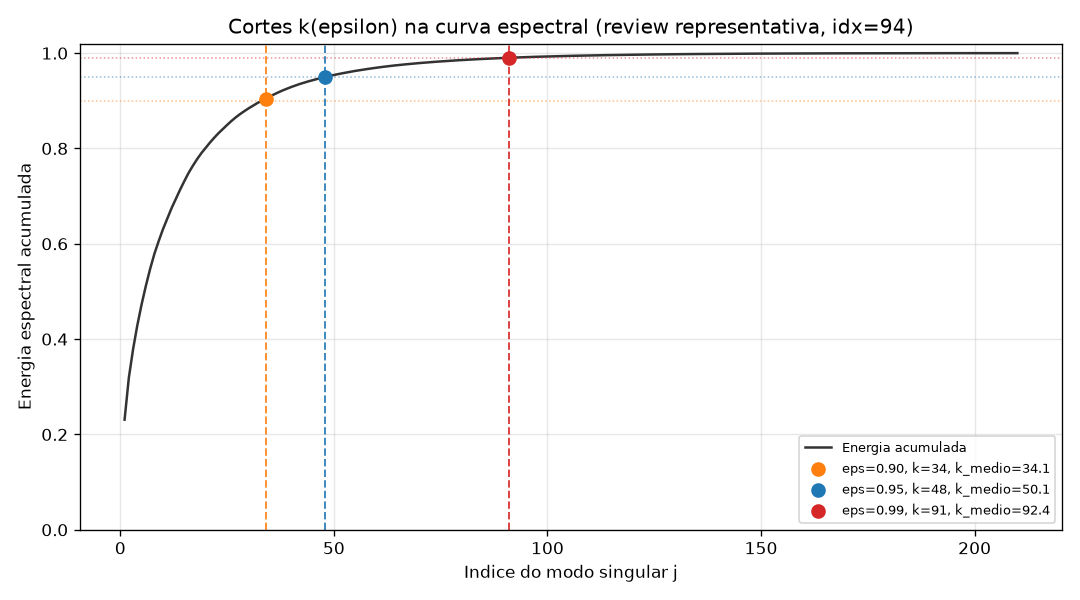
\includegraphics[width=0.92\linewidth]{figures/epsilon_k_cortes.png}
    \caption{Energia espectral acumulada de uma review representativa e pontos de corte $k(\varepsilon)$ para $\varepsilon \in \{0{,}90, 0{,}95, 0{,}99\}$. Anotações incluem $\bar{k}$ médio no corpus.}
    \label{fig:epsilon-k}
\end{figure}

\begin{table}[ht]
    \centering
    \caption{$\bar{k}$, $E_k^{\mathrm{energia}}$ e $\bar{R}_k$ para \texttt{svd} por $\varepsilon$ (média no corpus; invariantes a $\rho$).}
    \label{tab:metricas-eps}
    \small
    \begin{tabular}{lccc}
        \hline
        $\varepsilon$ & $\bar{k}$ & $E_k^{\mathrm{energia}}$ & $\bar{R}_k$ \\
        \hline
        0,90 & 34,1 & 0,903 & 0,688 \\
        0,95 & 50,1 & 0,951 & 0,779 \\
        0,99 & 92,4 & 0,990 & 0,901 \\
        \hline
    \end{tabular}
\end{table}

\subsection{Compressão e acurácia downstream}

Com $\bar{T}\approx 209$ tokens por review, o corpus permite poda em sequências mais longas que em bases de notícias curtas. Mesmo em $\rho=0{,}125$, mantém-se em média $\bar{T'}\approx 26$ tokens por review. A acurácia downstream situa-se entre $\approx 0{,}68$ e $0{,}79$. As Tabelas~\ref{tab:imdb-e90} a \ref{tab:imdb-e99} detalham os resultados por $\varepsilon$; a Figura~\ref{fig:tradeoff} resume o trade-off acurácia $\times$ compressão.

Destaques:
\begin{itemize}
    \item \textbf{Melhor configuração}: \texttt{svd}, $\varepsilon=0{,}99$, $\rho=0{,}50$, com acurácia 0,792, acima da referência sem poda (0,750) neste proxy.
    \item \textbf{Efeito de $\varepsilon$ em \texttt{svd}}: para $\rho=0{,}50$, a acurácia passa de 0,750 ($\varepsilon=0{,}90$) para 0,783 ($\varepsilon=0{,}95$) e 0,792 ($\varepsilon=0{,}99$); para $\rho=0{,}125$, de 0,683 para 0,725.
    \item \textbf{Baseline \texttt{random}}: em $\rho=0{,}25$, atinge 0,775, empatando com o melhor \texttt{svd}; em $\rho=0{,}125$, fica em 0,700 frente a 0,725 de \texttt{svd} no melhor $\varepsilon$.
    \item \textbf{Leitura}: o ganho de \texttt{svd} depende do orçamento $\rho$ e da riqueza do subespaço ($\varepsilon$); \texttt{random} não varia com $\varepsilon$.
\end{itemize}

\begin{figure}[ht]
    \centering
    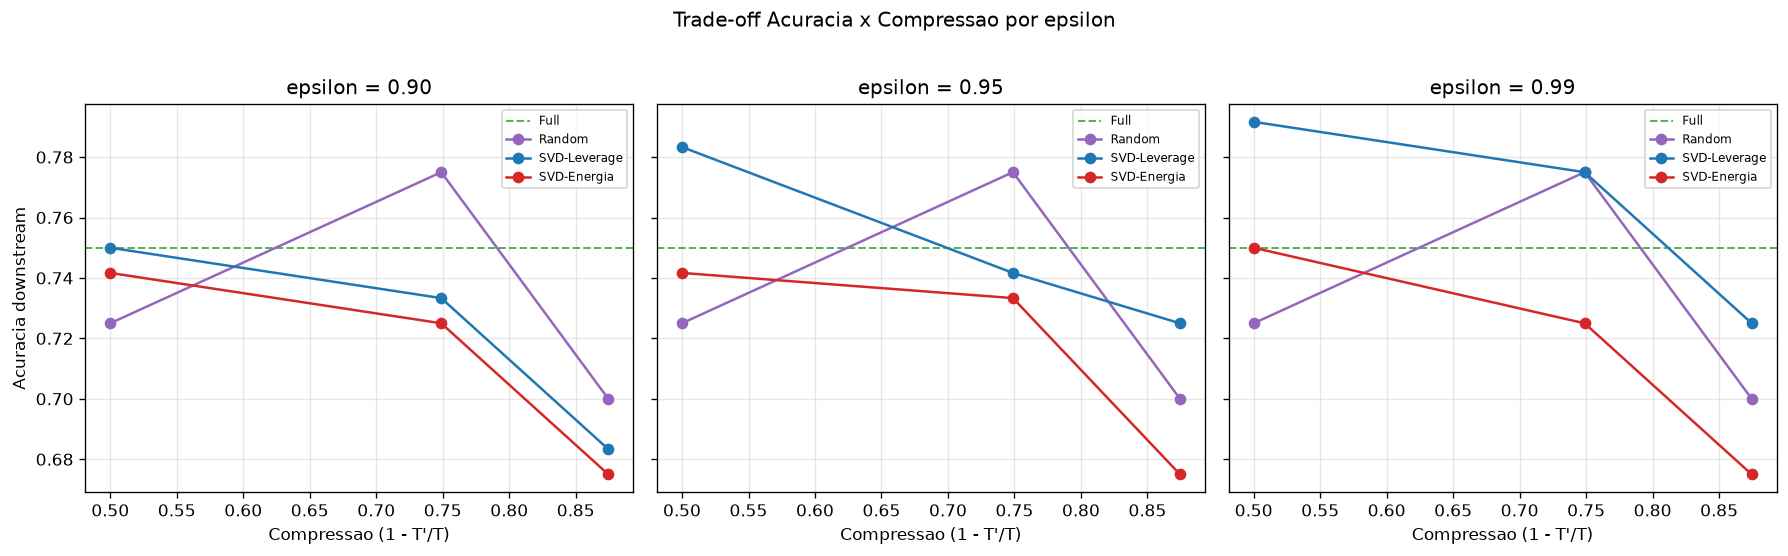
\includegraphics[width=\linewidth]{figures/tradeoff_acerto_compressao.png}
    \caption{Acurácia downstream $\times$ compressão (IMDb), facetada por $\varepsilon$. Cada painel compara os quatro métodos nos três níveis de $\rho$.}
    \label{fig:tradeoff}
\end{figure}

\begin{table}[ht]
    \centering
    \caption{Acurácia downstream por método e $\rho$ com $\varepsilon=0{,}90$.}
    \label{tab:imdb-e90}
    \small
    \begin{tabular}{lccc}
        \hline
        Método & $\rho=0{,}50$ & $\rho=0{,}25$ & $\rho=0{,}125$ \\
        \hline
        full & 0,750 & 0,750 & 0,750 \\
        random & 0,725 & 0,775 & 0,700 \\
        svd & 0,750 & 0,733 & 0,683 \\
        svd\_energia & 0,742 & 0,725 & 0,675 \\
        \hline
    \end{tabular}
\end{table}

\begin{table}[ht]
    \centering
    \caption{Acurácia downstream por método e $\rho$ com $\varepsilon=0{,}95$.}
    \label{tab:imdb-e95}
    \small
    \begin{tabular}{lccc}
        \hline
        Método & $\rho=0{,}50$ & $\rho=0{,}25$ & $\rho=0{,}125$ \\
        \hline
        full & 0,750 & 0,750 & 0,750 \\
        random & 0,725 & 0,775 & 0,700 \\
        svd & 0,783 & 0,742 & 0,725 \\
        svd\_energia & 0,742 & 0,733 & 0,675 \\
        \hline
    \end{tabular}
\end{table}

\begin{table}[ht]
    \centering
    \caption{Acurácia downstream por método e $\rho$ com $\varepsilon=0{,}99$.}
    \label{tab:imdb-e99}
    \small
    \begin{tabular}{lccc}
        \hline
        Método & $\rho=0{,}50$ & $\rho=0{,}25$ & $\rho=0{,}125$ \\
        \hline
        full & 0,750 & 0,750 & 0,750 \\
        random & 0,725 & 0,775 & 0,700 \\
        svd & 0,792 & 0,775 & 0,725 \\
        svd\_energia & 0,750 & 0,725 & 0,675 \\
        \hline
    \end{tabular}
\end{table}

\subsection{Pooling médio e poda moderada}\label{sec:pooling-poda}

Em $\rho=0{,}50$ e $\varepsilon=0{,}99$, \texttt{svd} supera levemente \texttt{full} (0,792 vs.\ 0,750; Tabela~\ref{tab:imdb-e99}). Não interpretamos isso como generalização \emph{cross-corpus}: a SVD é por documento e não supervisionada. A hipótese mais plausível, dado o protocolo de avaliação (Seção~\ref{sec:protocolo-clf}), é que a \textbf{poda melhore o pooling médio} usado como representação da review.

Com \texttt{full}, agregamos $\bar{T}\approx 209$ linhas de $F$ por média aritmética antes da normalização $L_2$ e do Ridge. Em reviews longas e redundantes, muitos subtokens contribuem pouco ao subespaço dominante da matriz --- enredo, repetições, trechos neutros --- mas entram com peso igual no pooling, \textbf{diluindo} o vetor agregado em $\mathbb{R}^D$. Com \texttt{svd} em $\rho=0{,}50$, mantêm-se $\bar{T'}\approx 105$ linhas ranqueadas por leverage no subespaço $F_k$; tokens de alta participação estrutural passam a pesar mais na média \emph{por exclusão} dos demais, produzindo um embedding de documento potencialmente mais \textbf{concentrado} para a tarefa de sentimento.

Dois elementos modulam essa leitura. Primeiro, o ganho de \texttt{svd} sobre \texttt{full} em $\rho=0{,}50$ só aparece claramente quando $\varepsilon$ é alto (0,750 em $\varepsilon=0{,}90$; 0,792 em $\varepsilon=0{,}99$): um subespaço $F_k$ mais rico ($\bar{k}\approx 92$) refina o ranqueamento antes da poda. Segundo, \texttt{random} também supera \texttt{full} em $\rho=0{,}25$ (0,775), o que indica que \textbf{reduzir o número de linhas agregadas} por si só pode ajudar neste proxy; o leverage acrescenta vantagem sobretudo em compressão mais agressiva ($\rho=0{,}125$) e quando $\varepsilon$ é elevado.
\subsection{Leitura algébrica dos métodos}

\texttt{svd} e \texttt{svd\_energia} compartilham a mesma decomposição singular, mas produzem rankings distintos:
\begin{itemize}
    \item \textbf{\texttt{svd}}: leverage clássico ($\ell_i/k$).
    \item \textbf{\texttt{svd\_energia}}: participação das linhas ponderada pelos valores singulares.
\end{itemize}
\texttt{svd\_energia} permanece abaixo de \texttt{svd} na maioria dos pares $(\varepsilon, \rho)$ e atinge 0,675 em $\rho=0{,}125$, independente de $\varepsilon$. Ponderar por $\Sigma_k$ concentra o ranking nos modos de maior energia; componentes menos dominantes podem ainda carregar sinal discriminativo para sentimento. Preservar energia espectral e preservar sinal downstream não coincidem necessariamente.

\subsection{Síntese dos achados}

Em relação às perguntas da Seção~\ref{sec:metodologia}:
\begin{enumerate}
    \item \textbf{Leverage score e acurácia}: a seleção por leverage mantém acurácia competitiva em compressão moderada; empata com \texttt{random} em $\rho=0{,}25$ (0,775) e supera em $\rho=0{,}125$ (0,725 vs.\ 0,700).
    \item \textbf{\texttt{svd\_energia} vs.\ \texttt{svd}}: a variante ponderada difere de \texttt{svd} e piora em $\rho$ baixo.
    \item \textbf{Invariância espectral a $\rho$}: $E_k^{\mathrm{energia}}$, $\bar{R}_k$ e $\bar{k}$ variam com $\varepsilon$ e permanecem invariantes a $\rho$ (Tabela~\ref{tab:metricas-eps}); medem $F_k$, não $S$.
\end{enumerate}

No proxy IMDb, $\varepsilon$ define o subespaço $F_k$, os leverage scores convertem esse subespaço em importância por token, e $\rho$ aplica a poda. A comparação com \texttt{svd\_energia} indica que maximizar energia espectral nos modos dominantes não coincide com maximizar utilidade supervisionada.

\section{Conclusão}\label{sec:conclusao}

Implementamos e avaliamos compressão token-level via SVD truncada e leverage scores em reviews IMDb, isolando um operador algébrico por documento (Seções~\ref{sec:metodologia}--\ref{sec:resultados}). Conforme a Seção~\ref{sec:resultados}, métricas espectrais ($E_k^{\mathrm{energia}}$, $\bar{R}_k$, $\bar{k}$) caracterizam o subespaço truncado $F_k$, enquanto a poda efetiva depende de $(\varepsilon, \rho)$ e do critério de ranking entre \texttt{svd} e \texttt{svd\_energia}. Privilegiar modos de maior energia espectral não garante preservar sinal útil para a tarefa supervisionada --- em linha com o limite teórico entre reconstrução ótima em $\|\cdot\|_F$ e desempenho downstream (Seção~\ref{sec:fundamentacao}). Trata-se de avaliação de operador algébrico em proxy controlado, não de equivalência com poda em LLM end-to-end.

\paragraph{Limitações.}
O escopo restringe-se a um corpus IMDb ($\approx$400 amostras), encoder \texttt{all-MiniLM-L6-v2} fixo e avaliação via pooling médio com classificador ridge --- proxies que colapsam a sequência e não medem qualidade generativa. As diferenças de acurácia entre métodos são modestas e não foram acompanhadas de testes de significância estatística.

Do ponto de vista de ALC, o trabalho percorre o encadeamento ortogonalização e mudança de base (Gram--Schmidt) \cite{alc11base}, teorema espectral e PSD de $F^\top F$ \cite{alc19espectral}, SVD retangular e posto efetivo \cite{alc21svd,alcposto}, até leverage scores como participação das linhas no subespaço dominante, com produto interno e normas \cite{alc04produto} subjacentes ao ranqueamento.

\paragraph{Trabalhos futuros.}
Dois eixos naturais de extensão: (i)~aplicar SVD no nível de \emph{content}/chunk em sumarizações produzidas por modelo de sentença, usando leverage ou similaridade entre embeddings de trechos para extrair os principais corpos quando há redundância entre conteúdos; (ii)~seleção \emph{query-aware}, combinando score estrutural (SVD/leverage) com similaridade ao embedding da consulta \cite{zhang2026fastcontext,alc04produto}.


\section*{Código}\label{sec:codigo}
O código que acompanha este relatório está disponível em:
\url{https://github.com/thiago-ouverney/svd-leverage-token-compression}.
Execução: \texttt{python experimento.py --max-amostras 400 --max-tokens 256}.
Saídas consumidas pelo artigo: \texttt{resultados/resultados.csv} e \texttt{resultados/tradeoff\_acerto\_compressao.png}.

\bibliography{refs}
\end{document}
